\chapter{The Compact Muon Solenoid Detector}
\label{chap:CMS}

\begin{figure}[tbh!]
 \begin{center}
 \begin{tabular}{c}
 \includegraphics[width=0.8\textwidth]{figures/Part2/CMS/cms}
 \end{tabular}
 \caption{A cutaway view of the \ac{CMS} detector. Adapted from~\cite{Sakuma:2013jqa}.}
 \label{fig:CMS}
 \end{center}
\end{figure}

\section{Coordinate System Used in the CMS Detector}

\begin{figure}[tbh!]
 \begin{center}
 \begin{tabular}{c}
 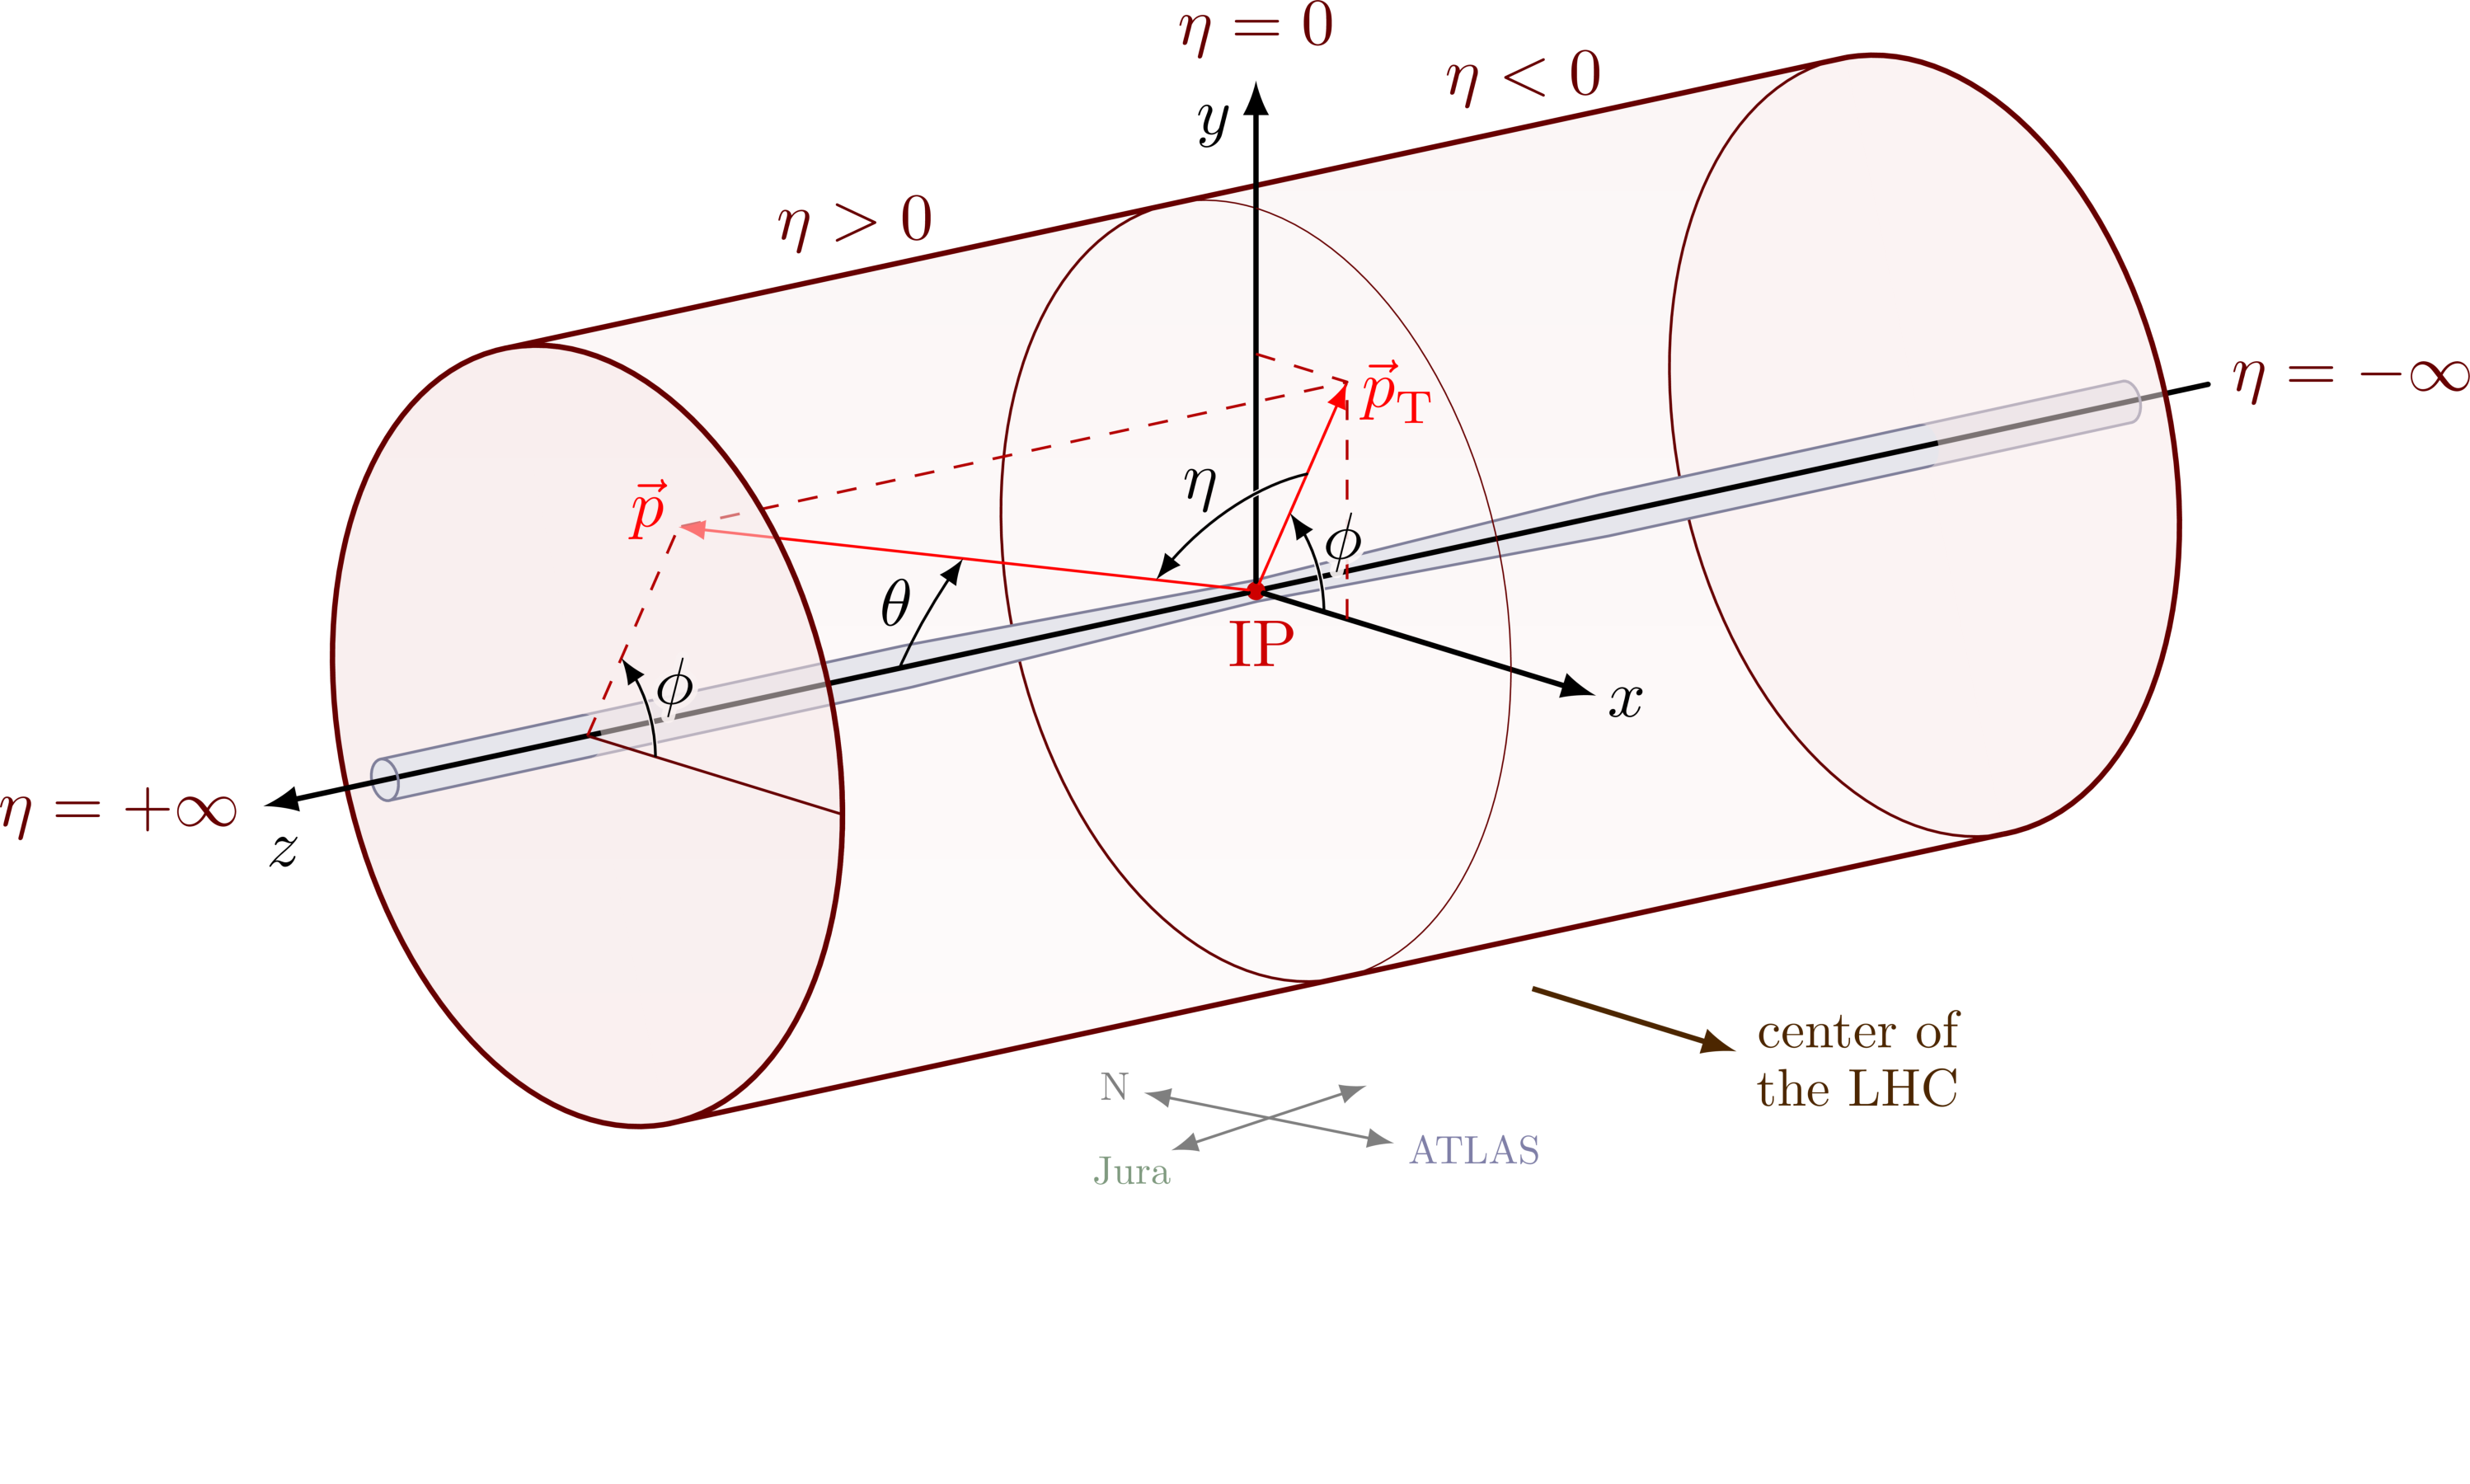
\includegraphics[width=0.8\textwidth]{figures/Part2/CMS/axis3D_CMS-004}
 \end{tabular}
 \caption{A cutaway view of the \ac{CMS} detector. Adapted from~\cite{tikz:3D}.}
 \label{fig:axis3D}
 \end{center}
\end{figure}

\begin{figure}[tbh!]
 \begin{center}
 \begin{tabular}{c}
 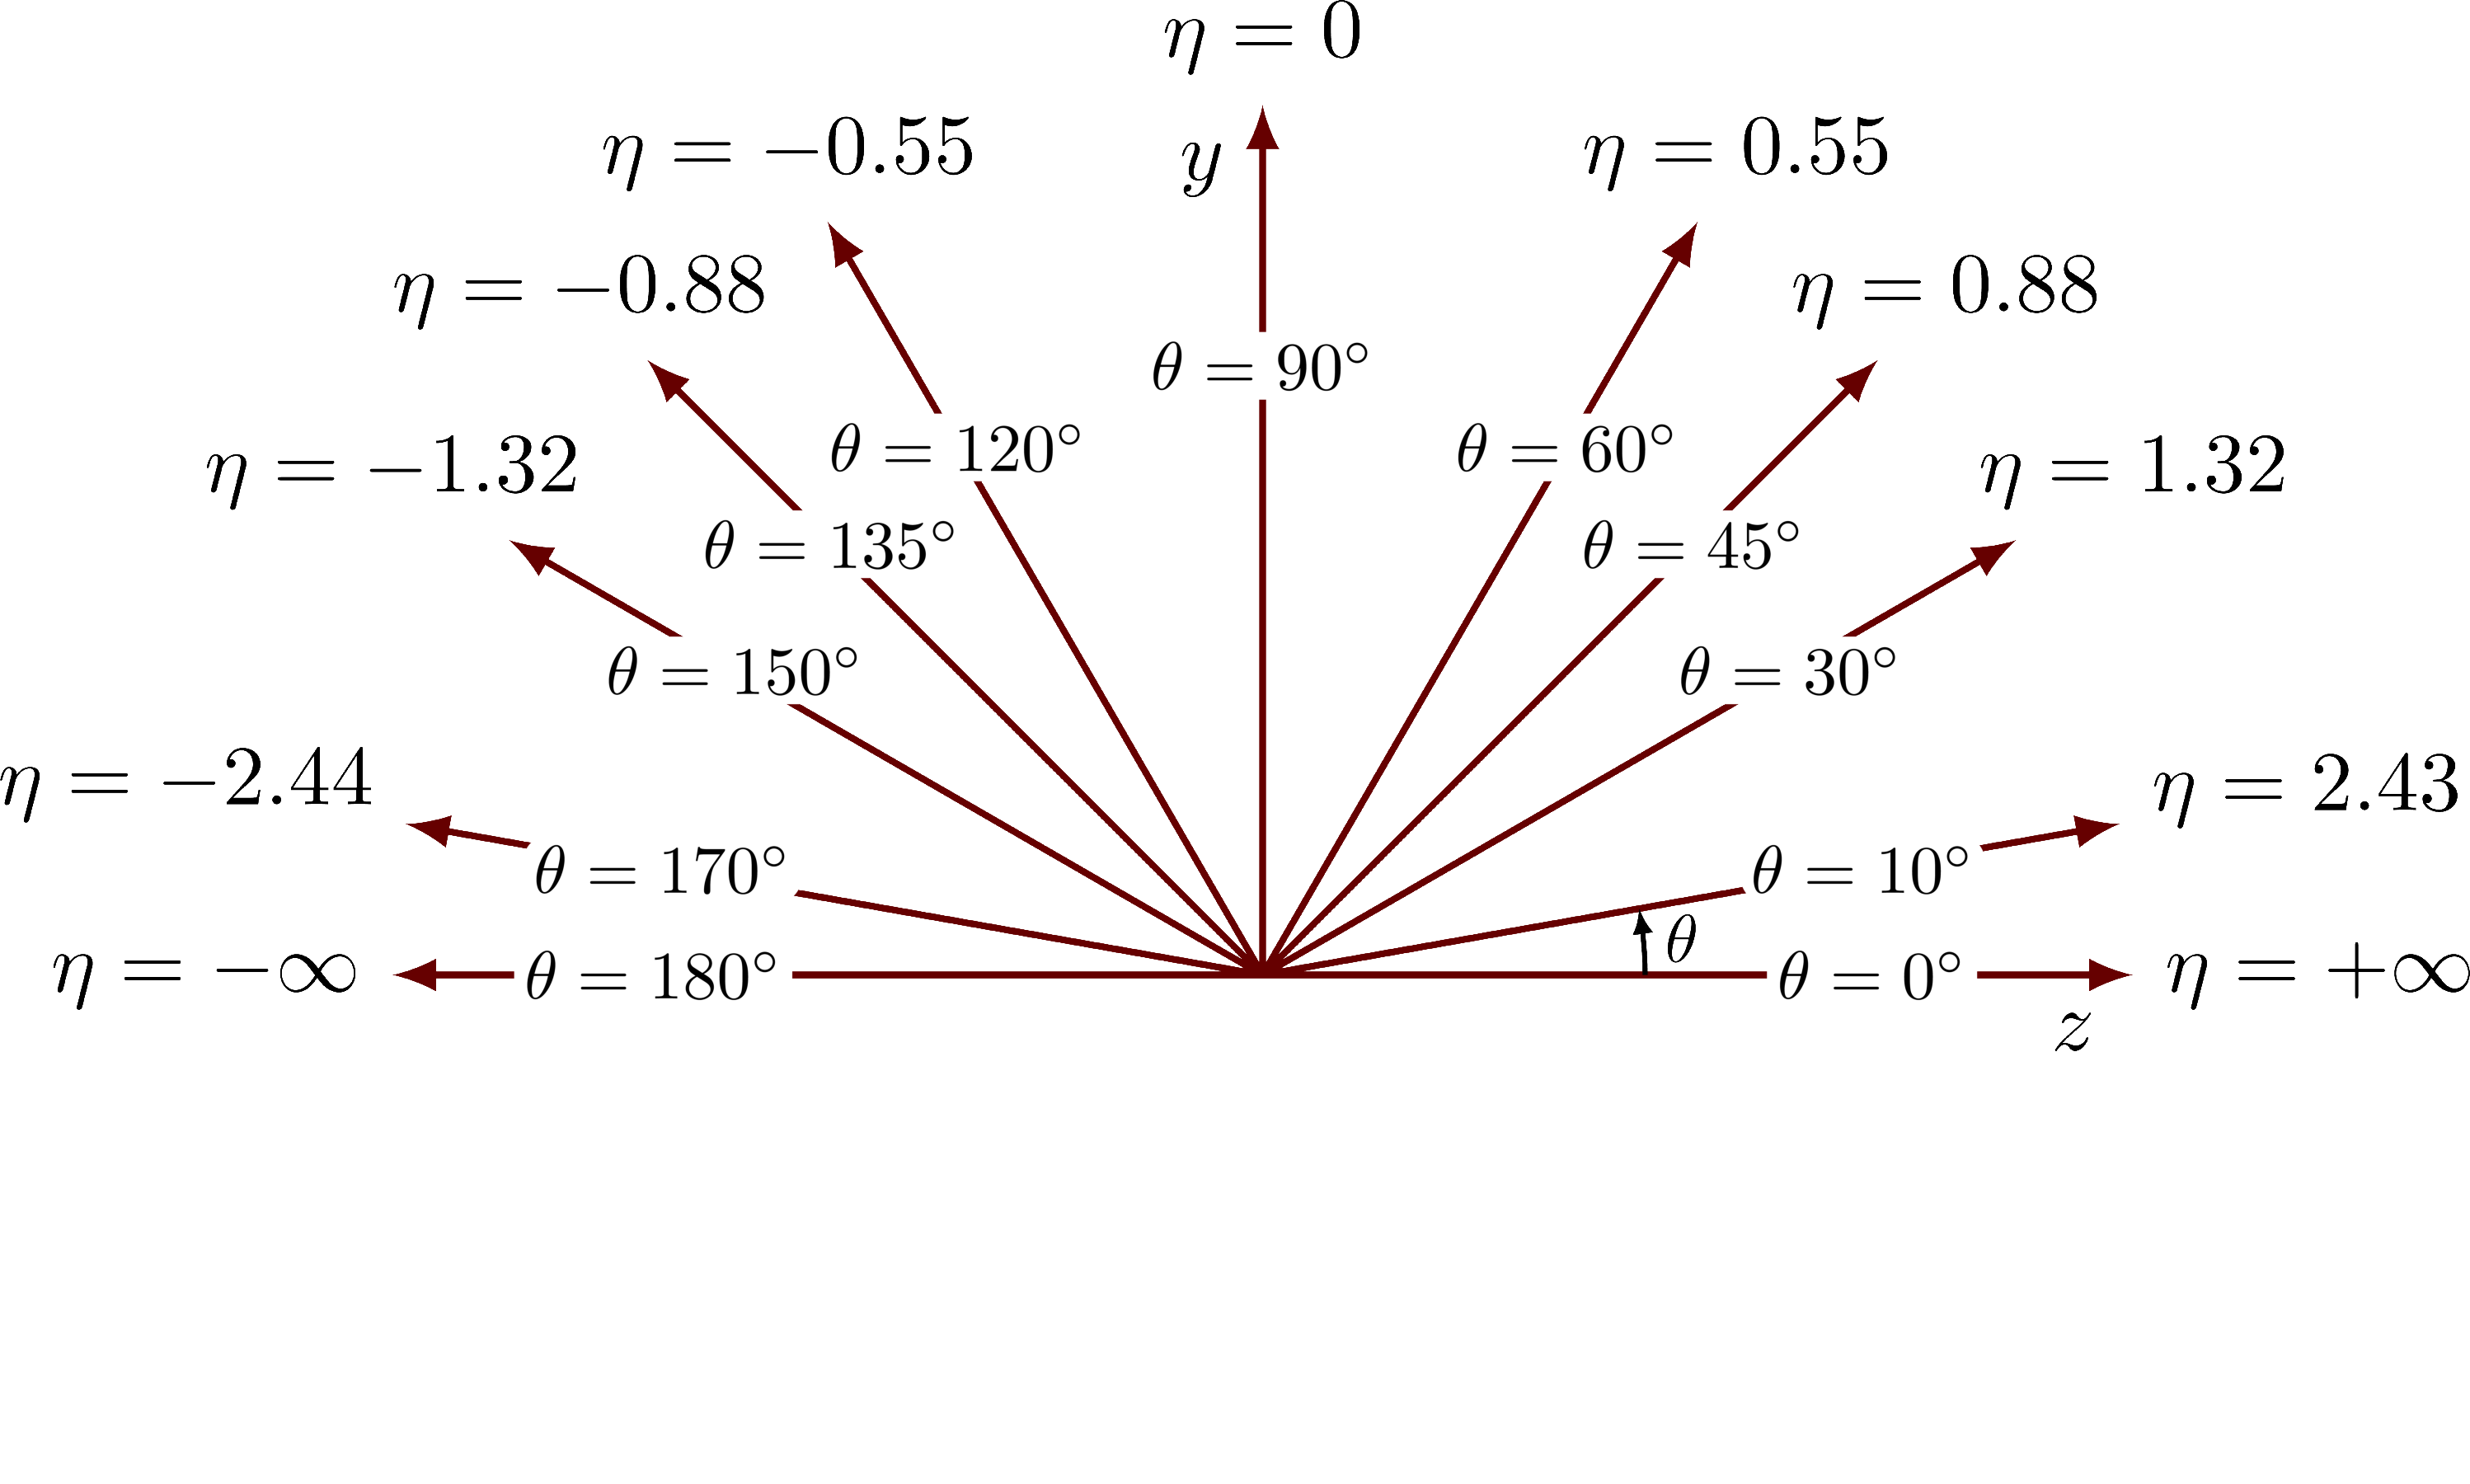
\includegraphics[width=0.8\textwidth]{figures/Part2/CMS/axis2D_pseudorapidity-003}
 \end{tabular}
 \caption{A cutaway view of the \ac{CMS} detector. Adapted from~\cite{tikz:2D}.}
 \label{fig:axis2D}
 \end{center}
\end{figure}

\section{The Inner Tracking System}

\section{The Electromagnetic Calorimeter}

\section{The Hadronic Calorimeter}

\section{The Superconducting Magnet}

\section{The Muon System}

\section{The Trigger System}